\documentclass[revision-guide.tex]{subfiles}
%% Current Author: BC
\setcounter{chapter}{5}
\begin{document}
\chapter{Waves}
\begin{content}
\item progressive waves
\item longitudinal and transverse waves
\item electromagnetic spectrum
\item polarisation
\item refraction
\end{content}

\section*{Candidates should be able to:}
\spec{understand and use the terms displacement, amplitude, intensity, frequency, period, speed and wavelength}

All waves consist of oscillations. The oscillations could be of particles, for example in a sound wave, or of an electromagnetic field, as in a light wave.

The following terms are used to describe properties of waves:
\begin{itemize}
\item \textbf{displacement}: This is a measurement of the distance and direction away from the equilibrium position.
\item \textbf{amplitude}: The maximum displacement of the oscillation, represented by $A$.
\item \textbf{intensity}: The power of the wave per unit area, represented by $I$. The unit of intensity is $Wm^{-2}$.
\item \textbf{frequency}: The number of oscillations per second, represented by $f$.
\item \textbf{period}: The time taken for one oscillation, represented by $T$.
\item \textbf{speed}: The speed of a wave represented by $v$. This will depend on the medium through which the wave is travelling.
\item \textbf{wavelength}: The distance over which a wave's shape repeats, represented by $\lambda$.

\end{itemize}

\spec{recall and apply $f = \frac{1}{T}$ to a variety of situations not limited to waves}

This equation follows from the definition of the frequency and time period of a wave. Remember to use Hertz as the unit for frequency and seconds as the unit for period. 

\spec{recall and use the wave equation $v=f\lambda$}

$$speed = \frac{distance travelled}{time taken}$$

For a wave, the distance travelled in one time period, $T$, is the wavelength, $\lambda$. Therefore we can write

\[v = \frac{\lambda}{T}\]

Then, using the equation $f=\frac{1}{T}$, we can write:

$$v = f\lambda$$

This is known as the wave equation and can be applied to all waves. The frequency of the wave generally depends on the source of the wave or how it is produced and the speed depends on the medium through which the wave is travelling.

\spec{recall that a sound wave is a longitudinal wave which can be described in terms of the displacement of molecules or changes in pressure}

When a sound wave travels through a material, the collisions of molecules are parallel to the direction of travel. Energy is transferred through these collisions and the speed of the sound wave will depend on factors such as the density of the material and the temperature.

When a sound wave is viewed on an oscilloscope, it looks as though the oscillations are perpendicular to the direction of travel, as in a transverse wave. The y-axis can represent either the displacement of molecules (still in the parallel direction) from their equilibrium position, or the difference in pressure.

\begin{figure}[h]
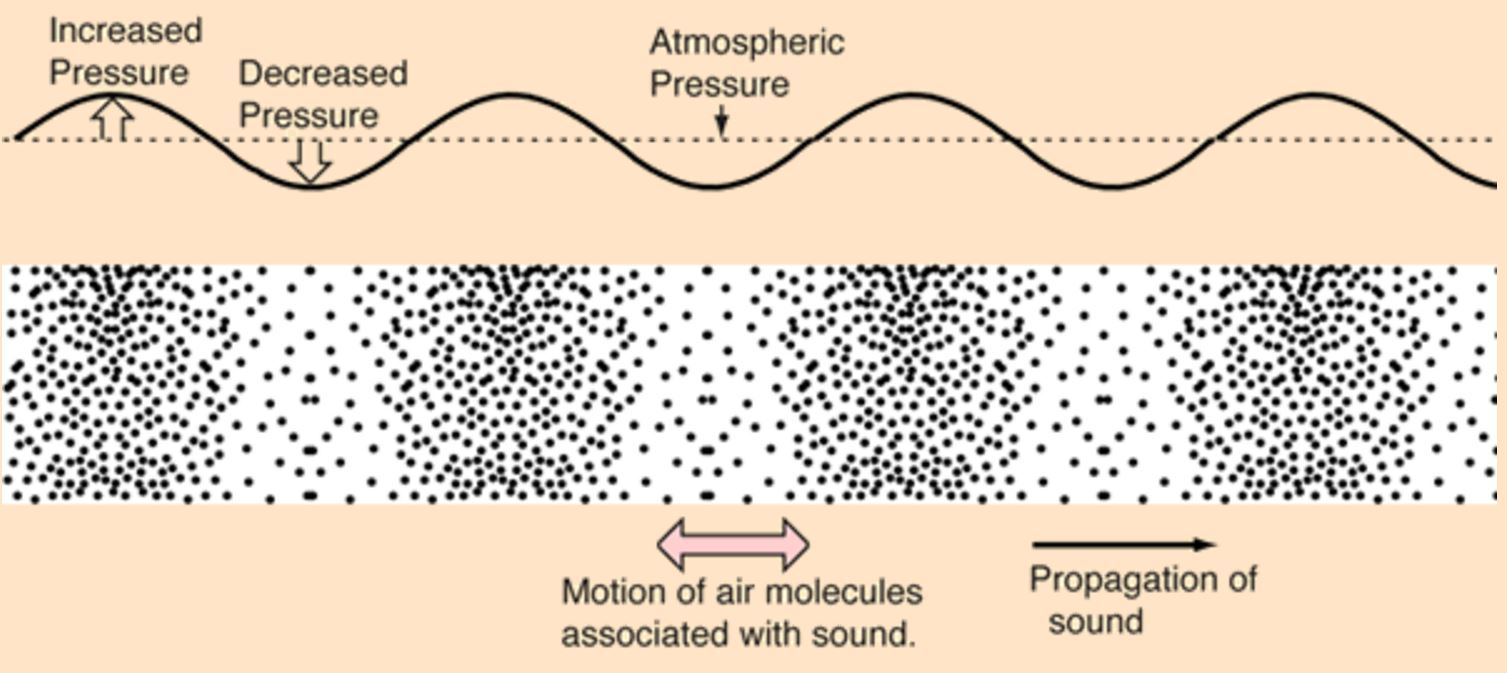
\includegraphics[width=\textwidth]{figs/chapt-6/soundwave.JPG}
\caption{Sound wave in air (credit: hyperphysics)}
\label{Sound wave in air}
\end{figure}

\spec{recall that light waves are transverse electromagnetic waves, and that all electromagnetic waves travel at the same speed in a vacuum}
\spec{recall the major divisions of the electromagnetic spectrum in order of wavelength, and the range of wavelengths of the visible spectrum}

Electromagnetic waves are transverse waves where the oscillations are perpendicular to the direction of travel. In all electromagnetic waves there are actually two waves oscillating perpendicular to each other and to the direction of travel. One is an oscillating magnetic field; the other an oscillation electric field.

\begin{figure}[h!]
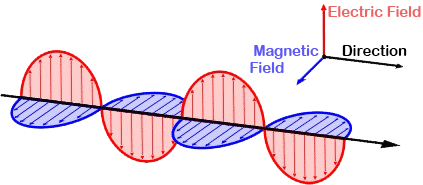
\includegraphics[width=9cm]{figs/chapt-6/emwave.png}
\centering
\caption{oscillations in an electromagnetic wave}
\label{emwave}
\end{figure}

The electromagnetic spectrum is the name for the arrangement and classification of electromagnetic waves in order of their wavelengths or frequencies.

The electromagnetic spectrum is shown below in order of increasing wavelength.

\begin{figure}[h]
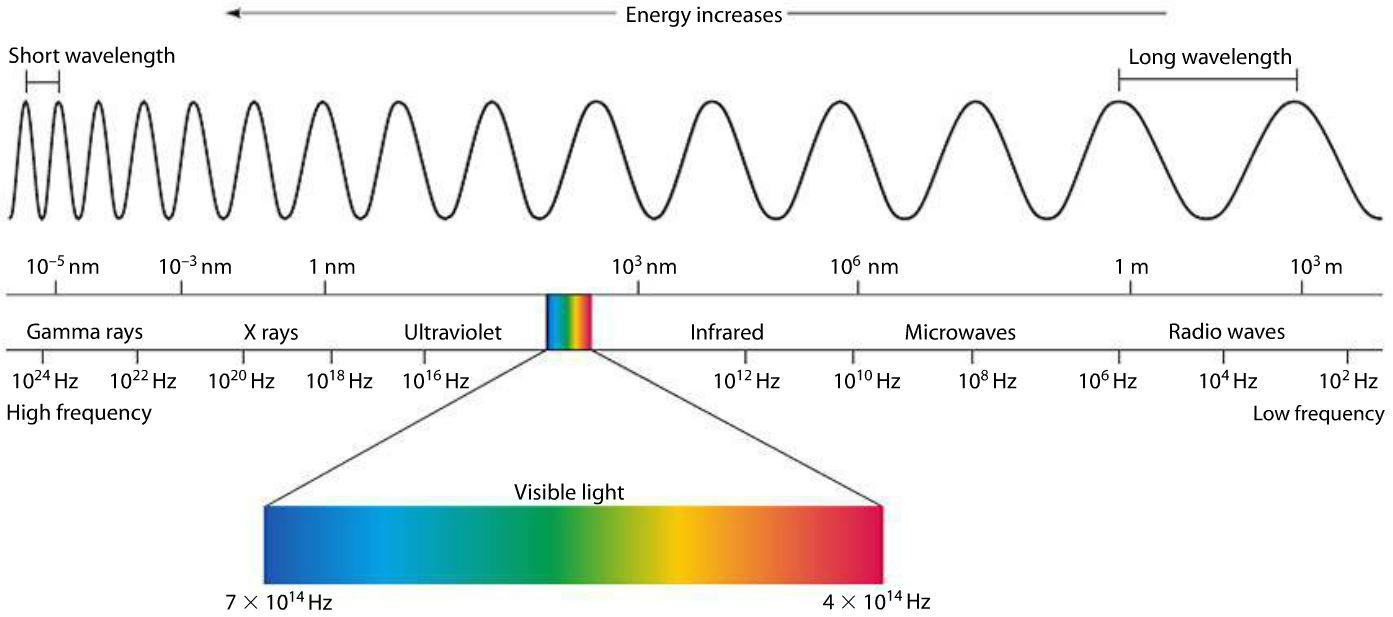
\includegraphics[width=\textwidth]{figs/chapt-6/emspectrum.jpg}
\caption{The electromagnetic spectrum (Credit:miniphysics.com)}
\end{figure}

You can see that the visible light spectrum makes up a small part of the electromagnetic spectrum, with wavelengths between 400 - 700 nm.

\spec{recall that the intensity of a wave is directly proportional to the square of its amplitude}

If the amplitude of a wave varies sinusoidally, the intensity will vary as sine squared. Therefore the following expression can be used:

$$I \propto A^2$$

\spec{use graphs to represent transverse and longitudinal waves, including standing waves}

\emph{Note: Standing waves will be covered in Chapter 7 on Superposition}

There are two types of graphs used to represent transverse and longitudinal waves, shown in Figure \ref{twographs}. You need to be careful as they look similar.

The first graph plots the motion of one part of the wave with time, for example the motion of one water molecule as a water wave goes by. The x-axis on this graph can give you the time period of the wave.

The second graph is a snapshot of a section of the wave at one particular instant in time. On this graph the wavelength can be measured from the x-axis.

\begin{figure}[h]
    \begin{center}
    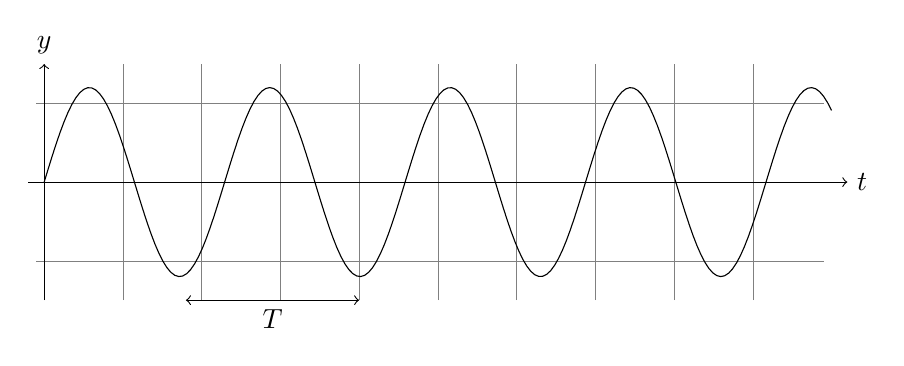
\begin{tikzpicture}[domain=0:10,samples=200]
        \draw[very thin,color=gray] (-0.1,-1.5) grid (9.9,1.5);
        \draw[->] (-0.2,0) -- (10.2,0) node[right] {$t$};
        \draw[->] (0,-1.5) -- (0,1.5) node[above] {$y$};
        \draw plot (\x,{1.2*sin(50*pi*\x)});
        \draw[<->] (1.8,-1.5) -- (4,-1.5) node[midway, below] {$T$};
    \end{tikzpicture}
    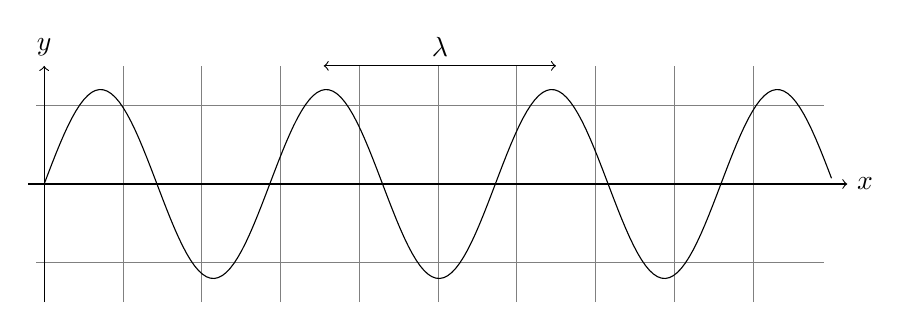
\begin{tikzpicture}[domain=0:10,samples=200]
        \draw[very thin,color=gray] (-0.1,-1.5) grid (9.9,1.5);
        \draw[->] (-0.2,0) -- (10.2,0) node[right] {$x$};
        \draw[->] (0,-1.5) -- (0,1.5) node[above] {$y$};
        \draw plot (\x,{1.2*sin(40*pi*\x)});
        \draw[<->] (3.55,1.5) -- (6.5,1.5) node[midway, above] {$\lambda$};
    \end{tikzpicture}
    \end{center}
    \caption{Two graphs of a wave}
    \label{twographs}
\end{figure}
        
    

\spec{explain what is meant by a plane-polarised wave}
\spec{recall Malus' Law ($I \propto \cos^2\theta $) and use it to calculate the amplitude and intensity of transmission through a polarising filter}

A plane-polarised wave is one where there is only \textbf{one} allowed direction of oscillation. This is only applicable to transverse waves where there are multiple allowed modes of oscillation which are all perpendicular to the direction of travel. A longitudinal wave cannot be polarised as there is already only one direction of oscillation - the direction parallel to that of travel. All electromagnetic waves can be polarised.

Consider visible light as an example of a polarised wave. There are 4 ways in which light can be polarised.

\begin{itemize}
\item\textbf{Transmission}: A polarising filter can be used to polarise light. A filter is made up of chains of molecules that will absorb one direction of oscillation of the light wave, therefore only letting through the perpendicular direction. Note that this 'one' direction is a simplificiation as it encompasses oscillations in both the electric and magnetic fields. The \emph{axis of transmission} of a filter is the direction of oscillation that the filter will let through.

\begin{figure}[h]
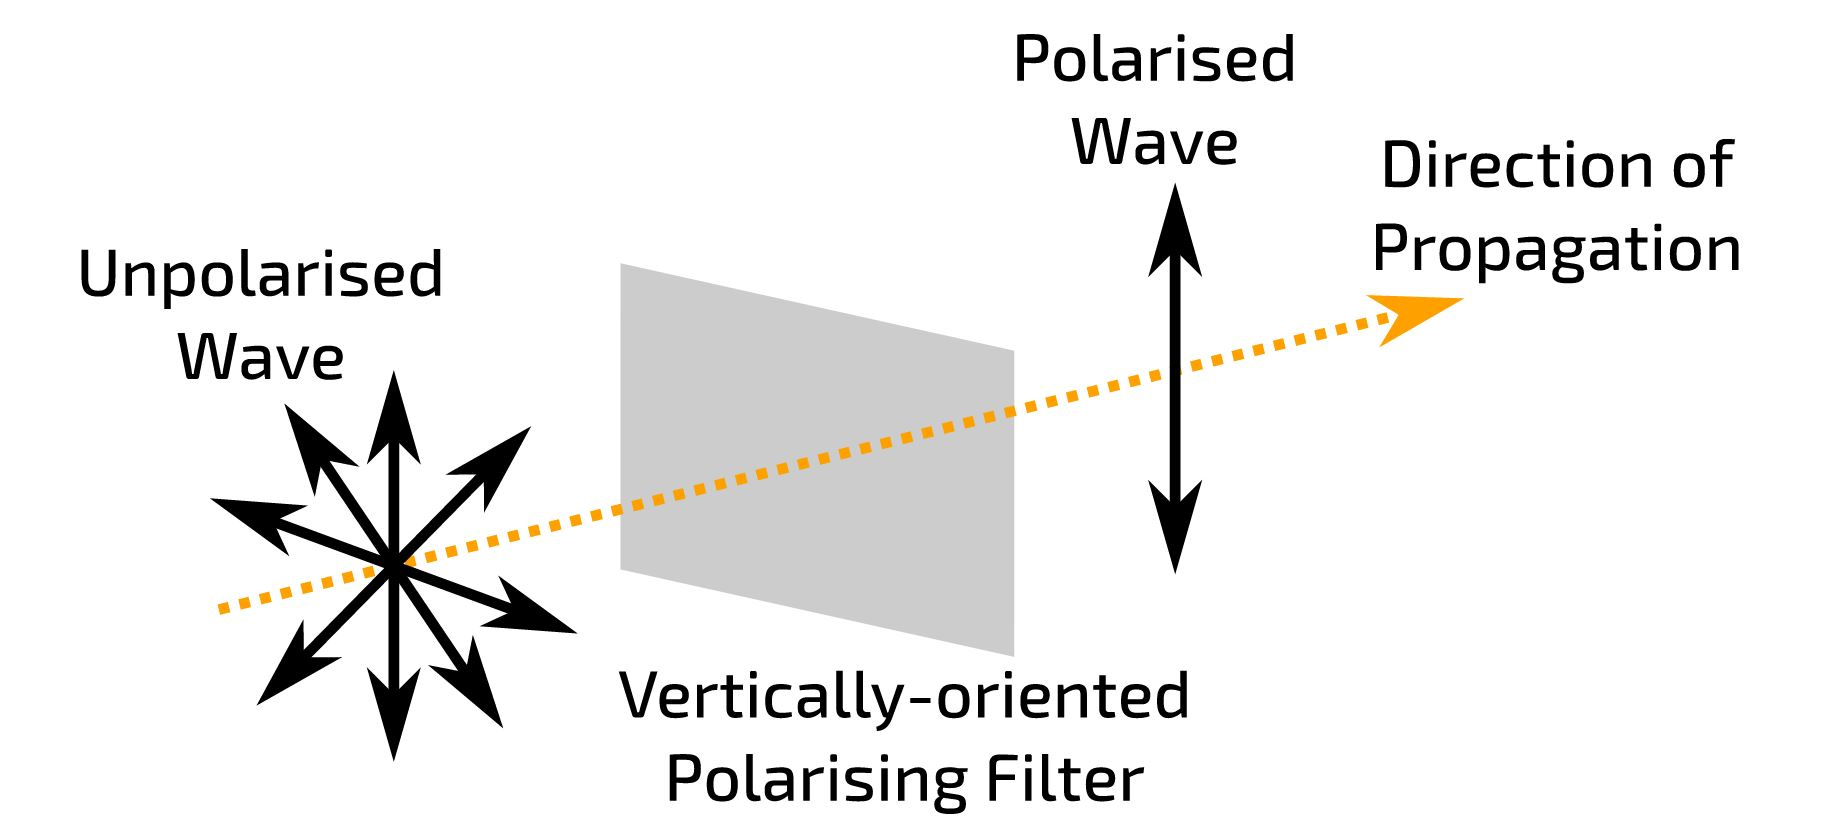
\includegraphics[width=10cm]{figs/chapt-6/polarisedwave.JPG}
\centering
\caption{diagram showing the operation of a polarising filter (Credit: isaacphysics)}
\end{figure}

As unpolarised light passes through a polaroid filter, its intensity will drop of 50\% of what it originally was. If light that is already polarised is incident on a filter with a perpendicular axis of transmission, none will pass through. If light that is already polarised is incident on a filter with a parallel axis of transmission, then all of the light will pass through. For cases other than parallel or perpendicular, Malus' Law can be used.

Malus' Law can be used to work out how the intensity of polarised light changes as it passes through a polaroid filter. The angle $\theta$ is the angle \emph{between} the direction of polarisation of the incident light and the axis of transmission of the polaroid. If you start with unpolarised light, $\theta$ is the angle between the two polaroids.

Malus' Law states that the intensity of the transmitted light is proportional to the square of $\cos\theta$.
$$I \propto \cos^2\theta $$
If the incident intensity is $I_0$, then we can write Malu's Law as:
$$I = I_0\cos^2\theta$$

Note that if you are dealing with \emph{amplitude} instead of intensity then you must take the square root to give $\cos\theta$.

\item\textbf{Reflection}: Light can be partially polarised on reflection from certain non metallic surfaces, such as water. The reflected light will be polarised parallel to the surface. This is why polaroid sunglasses are useful as they can cut out the glare from water or roads.

\item\textbf{Refraction}: Light can be partially polarised, often in two perpendicular directions, when passing through some materials, such as calcite. Specific details will always be given to you in a question.

\item\textbf{Scattering}: Light from the Sun scatters of molecules in our atmosphere and is partially polarised depending on the direction that you are looking at the sky. Again, specific details will always be provided in a question.

\end{itemize}

\spec{recognise and use the expression for refractive index
\[ n = \frac{\sin{\theta_1}}{\sin{\theta_2}} = \frac{v_1}{v_2}\]}

When a wave crosses a boundary which involves a change in speed, refraction occurs. This concept should be familiar from GCSE.

%Diagram

For light, the refractive index of a medium is the ratio of the speed of light in a vacuum, $c$, to the speed of light in the medium, $v$.
\[n = \frac{c}{v}\]

Therefore the refractive index of a material is always greater than one.

If a wave now crosses a boundary between material 1 and material 2, with the angle of incidence being $\theta_1$ and the angle of refraction being $\theta_2$, the following relationship (Snell's Law) applies:

\[ \frac{n_2}{n_1} = \frac{\sin{\theta_1}}{\sin{\theta_2}}\]

As the refractive index of a material is inversely proportional to the speed of light in that material, we know that

\[\frac{n_2}{n_1} = \frac{v_1}{v_2} \]

Snell's Law now becomes

\[ \frac{n_2}{n_1} = \frac{\sin{\theta_1}}{\sin{\theta_2}} =  \frac{v_1}{v_2}\]

This is the most general form of Snell's Law. For the specific case where material 1 is air we can take $n_1 = 1$ as the speed of light in air is so close to the speed of light in a vacuum. Now, replacing $n_2$ with $n$, the equation is:

\[ n = \frac{\sin{\theta_1}}{\sin{\theta_2}} = \frac{v_1}{v_2}\]

This is the equation given in the specification. Be careful as it only applies to the case where material 1 is air and this might not always be the case.

\spec{derive and recall $\sin{c} = \frac{1}{n}$ and use it to solve problems}

If we take Snell's Law for the case where light is travelling from a material of higher refractive index into a material with lower refractive index, $n_1 > n_2$, we know that the light will bend away from the normal with the angle of refraction, $\theta_2$ being larger than the angle of incidence, $\theta_1$. If the angle of incidence is increased until the angle of refraction is $90^{\circ}$, then the angle of incidence is now called the \emph{critical angle}, as above this angle, \emph{total internal reflection} will occur.

Now we can put this into Snell's Law. $\theta_1$ is now $c$, the critical angle and $\theta_2$ is now $90^{\circ}$.

$$\frac{n_2}{n_1} = \frac{\sin{\theta_1}}{\sin{\theta_2}}$$
This now becomes:
$$\frac{n_2}{n_1} = \frac{\sin{c}}{\sin{90^{\circ}}}$$

As $\sin{90^{\circ}} = 1$, the most general equation to find the critical angle is:
$$\frac{n_2}{n_1} = \sin{c}$$
or
$$\frac{n_1}{n_2} = \frac{1}{\sin{c}}$$

In the specification, the equation is given for the specific case where material 2 is air, therefore $n_2$ can be taken to be 1. This gives the equation: 
$$\sin{c} = \frac{1}{n}$$

\spec{recall that optical fibres use total internal reflection to transmit signals}
\spec{recall that, in general, waves are partially transmitted and partially reflected at an interface between media.}

Should be familiar from GCSE.

\end{document}
